% !TeX program = pdflatex
% !TeX encoding = UTF-8
% !TeX spellcheck = es_ES

\documentclass[9pt, handout]{beamer}

%********************************************************************
% Packages
%********************************************************************

\usepackage[utf8]{inputenc}
\usepackage[T1]{fontenc}
\usepackage[english]{babel}
\usepackage[bottom, para]{footmisc}
\usepackage{amsmath,amssymb,amsthm}
\usepackage{graphicx}
\usepackage{hyperref}
\usepackage{listings}
\usepackage{perpage}
\usepackage{xcolor}
\usepackage{wrapfig}
\usepackage{ifthen}
\usepackage{scrextend} % add margin to answers
\usepackage{dashrule}

%********************************************************************
% Packages options
%********************************************************************

% geometry
\usepackage{geometry}
\geometry{
    a4paper,
    ignoremp,
    bindingoffset = 1cm, 
    textwidth     = 13.5cm,
    textheight    = 21.5cm,
    lmargin       = 1cm,
    rmargin		    = 3cm,
    tmargin       = 2cm,
    bmargin       = 3cm
}

% listings
\renewcommand{\lstlistingname}{Code}

\definecolor{lightgray}{rgb}{.9,.9,.9}
\definecolor{darkgray}{rgb}{.4,.4,.4}
\definecolor{purple}{rgb}{0.65, 0.12, 0.82}
\lstset{
  basicstyle=\small\sffamily,
  numbers=left,
  numberstyle=\tiny,
  numbersep=3pt,
  stepnumber=1,
  frame=tb,
  columns=fullflexible,
  backgroundcolor=\color{yellow!15},
  keywordstyle=\color{blue}\bfseries,
  ndkeywordstyle=\color{darkgray}\bfseries,
  identifierstyle=\color{black},
  commentstyle=\color{purple}\ttfamily,
  stringstyle=\color{red}\ttfamily,
  numberbychapter=false,
  showstringspaces=false,
  breaklines=true,
  captionpos=b, % put captions at the bottom 
}
%\lstset{
%  numbersep=5pt,
%  frame=trbl
%}

\definecolor{prismgreen}{rgb}{0.12, 0.48, 0.12}
\lstdefinelanguage{prism}{ % syntax highlight via font
  keywords={
    bool,C,ceil,const,ctmc,double,dtmc,endinit,endmodule,endrewards,endsystem,F,false,floor,formula,G,global,I,init,int,label,max,mdp,min,module,nondeterministic,P,Pmin,Pmax,prob,probabilistic,R,rate,rewards,Rmin,Rmax,S,stochastic,system,true,U,X
  }, 
  keywordstyle={\bfseries\color{black}}, 
  numberstyle=\tiny\color{black}, 
  comment=[l] {//}, morecomment=[s]{/*}{*/}, % single and multi-line 
  commentstyle= \color{prismgreen}, % dark green 
  tabsize=4, % tab treatment (going to be fixed in Prism)
  escapechar=@ % write LaTeX comments escaped by @ symbol 
} 

% perpage
\MakePerPage{footnote}

% hyperref
\definecolor{webgreen}{rgb}{0,.5,0}
\definecolor{webbrown}{rgb}{.6,0,0}
\definecolor{RoyalBlue}{cmyk}{1, 0.50, 0, 0}
\hypersetup{%
  %draft, % = no hyperlinking at all (useful in b/w printouts)
  colorlinks=true, linktocpage=true, pdfstartpage=3, pdfstartview=FitV,%
  % uncomment the following line if you want to have black links (e.g., for printing)
  % colorlinks=false, linktocpage=false, pdfstartpage=3, pdfstartview=FitV, pdfborder={0 0 0},%
  breaklinks=true, pdfpagemode=UseNone, pageanchor=true, pdfpagemode=UseOutlines,%
  plainpages=false, bookmarksnumbered, bookmarksopen=true, bookmarksopenlevel=1,%
  hypertexnames=true, pdfhighlight=/O,%nesting=true,%frenchlinks,%
  urlcolor=RoyalBlue, linkcolor=black, citecolor=webbrown, %pagecolor=RoyalBlue,%
  %urlcolor=Black, linkcolor=Black, citecolor=Black, %pagecolor=Black,%
}

% graphicx
\graphicspath{{img/}}

%********************************************************************
% New commands
%********************************************************************

\newcommand{\question}[1]{%
  \vspace{20pt}%
  \begin{wrapfigure}{l}{0.1\textwidth}%
    \vspace{-30pt}%
    \begin{center}%
      
\includegraphics[scale=1]{hand.jpg}%
    \end{center}%
    \vspace{-30pt}%
  \end{wrapfigure}%
  \noindent #1%
}%
\newcommand{\answer}[1]{%
  \vspace{5pt}\par\noindent
  \textbf{\underline{Answer:}}%
  \begin{addmargin}[1em]{1em}% 1em left, 2em right
    #1%
    \begin{flushright}%
      \qedsymbol%
    \end{flushright}%
  \end{addmargin}%
}%

\definecolor{light-gray}{gray}{0.95}
\newboolean{inlineCodeBackground}
\setboolean{inlineCodeBackground}{false}
\newcommand{\prism}[1]{%
  \ifthenelse{\boolean{inlineCodeBackground}}{%
    \colorbox{light-gray}{\lstinline[language=prism]{#1}}%
  }{%
    \lstinline[language=prism]{#1}%
  }%
}%
\newcommand{\bash}[1]{%
  \ifthenelse{\boolean{inlineCodeBackground}}{%
    \colorbox{light-gray}{\lstinline[language=bash]{#1}}%
  }{%
    \lstinline[language=bash]{#1}%
  }%
}%

\newcommand{\dashedrule}{%
  \noindent\hdashrule{\textwidth}{1pt}{1.5mm}%
}%


\title[AAL y modelos aleatorios]{Ambient Assisted Living y modelos aleatorios}
\author{\textbf{Tommaso Papini}}
\institute{
  STLab, Departamiento de la Ingenieria de la Informacíon, Universidad de Florencia, Italia,\\
  {tommaso.papini@unifi.it}
}
\date{
  29 de Mayo 2017\\
  {\small Departamento de Informática, Universidad de Jaén, España}
}

\begin{document}

  \begin{frame}
    \titlepage
    \begin{itemize}
      \item Ambient Assisted Living
      \item Modelos y datasets
      \item Análisis de entornos inteligentes
    \end{itemize}
  \end{frame}

  \begin{frame}{Overview}
    %\tiny
    \tableofcontents
  \end{frame}
  
  \section{Ambient Assisted Living}
    
    \begin{frame}{Ambient Assisted Living}
      El \textbf{Ambient Assisted Living} es un sector de investigación que tiene como objetivo lo de ayudar las personas que viven en \textit{entornos inteligentes} (es decir, dotado de sensores y actuadores) explotando a la tecnología de sensores y de procesamiento de datos.
    \end{frame}
    
    \subsection{Objetivos}
      \begin{frame}{Objetivos}
        \pause
        Un \textit{entorno inteligente} es un sistema \textbf{parcialmente observable}:
        \pause
        \begin{itemize}
          \item el estado efectivo del sistema resulta oculto
          \pause
          \item solo se pueden observar eventos (\textit{observaciones}) emitidos por el sistema (por ej. la activación de un sensor)\\[1em]
        \end{itemize}
        
        \pause
        
        Principales análisis de interese:
        \pause
        \begin{itemize}
          \item \textbf{Diagnosis}: estimar cual es el estado efectivo actual del sistema a partir de las observaciones registradas
          \pause
          \item \textbf{Predicción}: estimar cual será el estado efectivo del sistema después de una determinada cantidad de tiempo
          \item \textbf{Planificación de acciones}: elegir la acción optima y entre cuanto tiempo ir actuarla para evitar situaciones críticas\\[1em]
        \end{itemize}
        
        \pause
        
        Análisis en linea:
        \pause
        \begin{itemize}
          \item la análisis en linea intenta analizar a un entorno inteligente \textit{mientras} está evolucionando
        \end{itemize}
      \end{frame}
    
  \section{Modelos y datasets}
    \subsection{Modelos estadísticos}
      \begin{frame}{Modelos estadísticos}
        Los \textit{modelos estadísticos} representan una aproximación de sistemas donde se modela:
        \begin{itemize}
          \item la evolución del estado del sistema
          \item parámetros estadísticos que definen como el sistema pasa de un estado al otro
        \end{itemize}
        \begin{center}
          \colorbox{white}{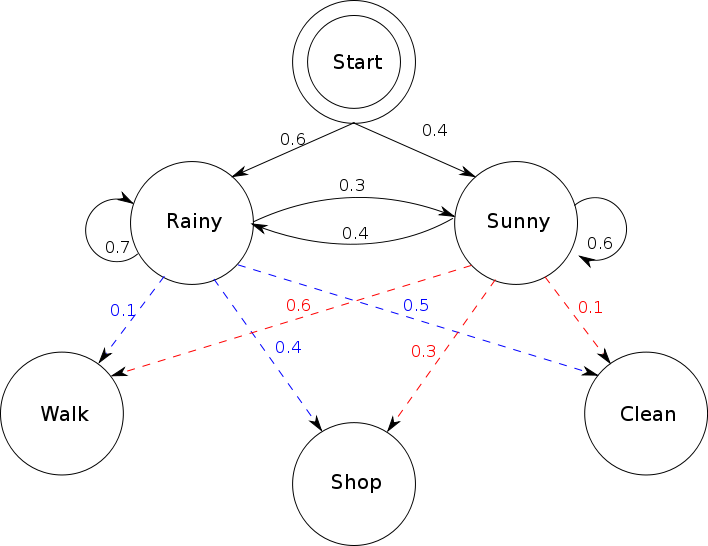
\includegraphics[scale=0.28]{708px-HMMGraph.png}}
        \end{center}
      \end{frame}
    
    \subsection{Datasets anotados}
      \begin{frame}{Datasets anotados}
        Un \textit{dataset anotado} es un dataset donde hay:
        \begin{itemize}
          \item los eventos registrados y cuando han pasado (marca temporal)
          \item anotaciones manuales de la evolución del estado efectivo del sistema (con intervalos temporales por cada estado)
        \end{itemize}
        Un ejemplo clásico de dataset anotado para AAL es el dataset de \textit{van Kasteren}\footnote{\url{https://sites.google.com/site/tim0306/datasets}}\footnote{Van Kasteren, T., Noulas, A., Englebienne, G. and Kröse, B., 2008, September. Accurate activity recognition in a home setting. In Proceedings of the 10th international conference on Ubiquitous computing (pp. 1-9). ACM.}\\[1em]
        
        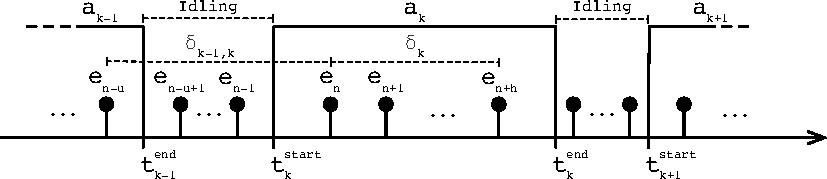
\includegraphics[scale=0.8]{activity_event_formulation.pdf}
      \end{frame}
    
    \subsection{Process mining}
      \begin{frame}{Process mining}{De datasets anotados a modelos estadísticos}
        Con el término \textbf{process mining} se indica un conjunto de técnicas para construir un modelo estadístico de un sistema parcialmente observable a partir de un dataset anotado de este mismo sistema.\\[1em]
        
        El process mining está compuesto por dos técnicas principales:
        \begin{itemize}
          \item \textbf{Process elicitation}: construye un modelo discreto (es decir, sin informaciones sobre la permanencia en los estados del sistema) a partir de los eventos y actividades anotados en el dataset
          \item \textbf{Process ehnancement}: añade una visión temporal continua a un modelo discreto introduciendo parámetros estadísticos que describen como el sistema evoluciona a lo largo del tiempo utilizando medidas estadísticas sacadas por el dataset
        \end{itemize}
      \end{frame}
    
  \section{Análisis de entornos inteligentes}
  
    \begin{frame}{Análisis de entornos inteligentes}{Esquema general}
      \begin{center}
        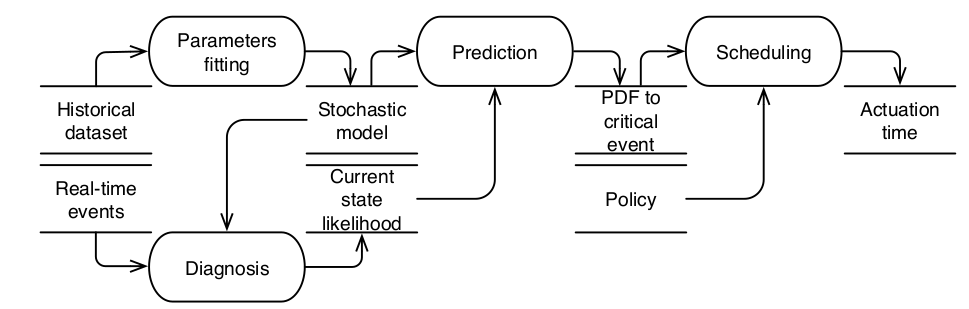
\includegraphics[scale=0.34]{architecture.png}
      \end{center}
      
      \begin{itemize}
        \item \textbf{Process mining}: de dataset anotado a modelo estadístico
        \item \textbf{Diagnosis}: de eventos efectivos a probabilidad del estado corriente (sobre un determinado modelo estadístico)
        \item \textbf{Predicción}: de probabilidad del estado corriente a probabilidad de que haya un evento crítico
        \item \textbf{Planificación}: de probabilidad de que haya un evento crítico a tiempo de respuesta (con una determinada política de respuesta)
      \end{itemize}
    \end{frame}
  
    \subsection{Diagnosis}
      \begin{frame}{Diagnosis}{Tiempo discreto}
        Los \textbf{Modelos Ocultos de Márkov} (Hidden Markov Model, HMM):
        \begin{itemize}
          \item modelan a un sistema parcialmente observable sin tener en cuenta del tiempo de permanencia en cada estado
          \item asocian a cada estado efectivo del sistema una distribución discreta sobre los eventos observables
          \item modelan a un sistema donde los estados efectivos evolucionan como una \textit{Cadena de Márkov Tiempo Discreto} (Discrete Time Markov Chain, DTMC)
          
        \end{itemize}
        \begin{center}
          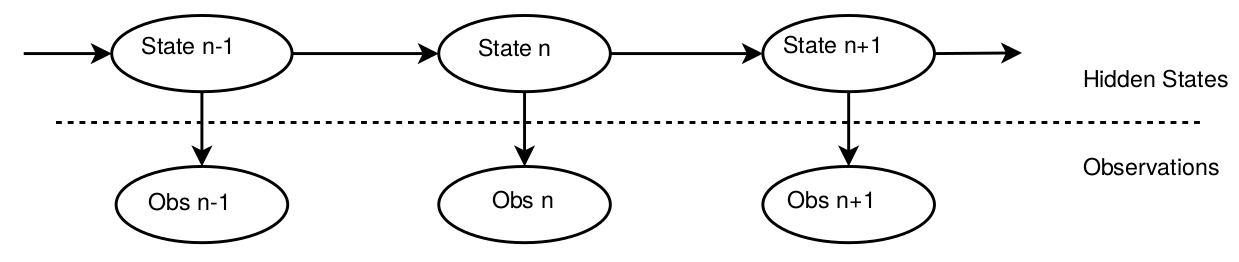
\includegraphics[scale=0.25]{HMM.png}
        \end{center}
        Diagnosis con HMM se puede lograr con algoritmos clásicos como el \textit{algoritmo de Viterbi} o el \textit{algoritmo de Forward-Backward}.
      \end{frame}
      
      \begin{frame}{Diagnosis}{Tiempo discreto con permanencia}
        \begin{itemize}
          \item \textbf{HSMM}\footnote{Van Kasteren, T.L.M., Englebienne, G. and Kröse, B.J., 2010. Activity recognition using semi-markov models on real world smart home datasets. Journal of ambient intelligence and smart environments, 2(3), pp.311-325.}
          \begin{itemize}
            \item Hidden Semi Markov Model
            \item permanencia en los estados ocultos modelada con distribuciones te tiempo discreto
            \item eventos generados en cada instante temporal
          \end{itemize}
          \item \textbf{IS-HSMM}/\textbf{ILP-HSMM}\footnote{Narimatsu, H. and Kasai, H., 2016. State Duration and Interval Modeling in Hidden Semi-Markov Model for Sequential Data Analysis. arXiv preprint arXiv:1608.06954.}
          \begin{itemize}
            \item Interval State-Hidden Semi Markov Model
            \item Interval Length Probability-Hidden Semi Markov Model
            \item extensiones de los HSMMs
            \item permite modelar a intervalos de silencio (es decir, sin eventos)
          \end{itemize}
        \end{itemize}
      \end{frame}
      
      \begin{frame}{Diagnosis}{Tiempo continuo}
        \begin{itemize}
          \item \textbf{HnMM}\footnote{Buchholz, R., Krull, C., Strigl, T. and Horton, G., 2010, March. Using hidden non-markovian models to reconstruct system behavior in partially-observable systems. In Proceedings of the 3rd International ICST Conference on Simulation Tools and Techniques (p. 86). ICST (Institute for Computer Sciences, Social-Informatics and Telecommunications Engineering).}
          \begin{itemize}
            \item Hidden nonMarkov Model
            \item tiempos de permanencia continuos
            \item cada \textit{transición} (es decir, el pasaje de un estado al siguiente) produce un evento
          \end{itemize}
          \item \textbf{GHSMM}\footnote{Salfner, F., 2006. Modeling event-driven time series with generalized hidden semi-Markov models.}
          \begin{itemize}
            \item Generalized Hidden Semi Markov Process
            \item tiempo de permanencia continuo
            \item solo una observación por cada estado
          \end{itemize}
        \end{itemize}
      \end{frame}
      
      \begin{frame}{Diagnosis}{H-MRGP-M}
        El \textbf{Modelo Oculto de un Proceso Regenerativo de Márkov} (Hidden-Markov Regenerative Process-Model) ha sido dessarollado por el STLab en la Universidad de Florencia.\footnote{Carnevali, L., Nugent, C., Patara, F. and Vicario, E., 2015, September. A continuous-time model-based approach to activity recognition for ambient assisted living. In International Conference on Quantitative Evaluation of Systems (pp. 38-53). Springer International Publishing.}
        
        \begin{itemize}
          \item Modela tiempo continuo de permanencia en los estados y del inter-tiempo entre eventos
          \item El estado del modelo evoluciona como un \textit{Proceso Regenerativo de Márkov} (Markov Regenerative Process, MRP)
        \end{itemize}
      \end{frame}
      
      \begin{frame}{Diagnosis}{H-MRGP-M}
        \begin{itemize}
          \item Experimentado sobre el dataset de van Kasteren
          \begin{itemize}
            \item 7+1 actividades
            \item \{Leaving house, Preparing a beverage, Preparing breakfast, Preparing dinner, Sleeping, Taking shower, Toileting\}
          \end{itemize}
          \item A partir de las marcas temporales en el dataset anotado, se calculan los tiempos continuos
          \begin{itemize}
            \item de permanencia en cada actividad
            \item de inter-tiempo entre eventos en cada actividad
          \end{itemize}
        \end{itemize}
        
    		\begin{table}[h!]
    			\centering
    			\small
    			\setlength{\tabcolsep}{5pt}
    			\def\arraystretch{0.75}
    			\begin{tabular}{| l | c | c || c | c |}
    				\hline
    				& \multicolumn{2}{|c||}{\bf Tiempo de permanencia}& \multicolumn{2}{|c|}{\bf Inter-tiempo entre eventos}\\
    				\cline{2-5}
    				& $\mu$ (s) & {\bf CV} & $\mu$ (s) & {\bf CV}\\
    				\hline
    				{\bf Leaving house} & 40\,261.455 & 1.042 & 9\,354.190 & 2.810 \\ \hline
    				{\bf Preparing a beverage} &  35.667 & 1.361 & 7.643 & 2.613\\ \hline
    				{\bf Preparing breakfast} &  108.684 & 0.713 & 9.928 & 1.844\\ \hline
    				{\bf Preparing dinner} &  1\,801.889 & 0.640 & 77.966 & 2.589\\ \hline
    				{\bf Sleeping} &  26\,116.571 & 0.442 & 1\,871.836 & 3.090\\ \hline
    				{\bf Taking shower} &  485.910 & 0.298 & 102.788 & 1.969\\ \hline
    				{\bf Toileting} &  88.742 & 1.175 & 14.814 & 2.449\\ 
    				\hline
      		\end{tabular}
    		\end{table}
      \end{frame}
      
      \begin{frame}{Diagnosis}{H-MRGP-M}
        El modelo H-MRGP-M es un \textit{modelo estadístico @runtime}
        \begin{itemize}
          \item El modelo se crea con técnicas de \textit{process mining}
          \begin{itemize}
            \item \textit{process elicitacion} para definir la topología del modelo
            \item \textit{process enhancement} para añadir parámetros estadísticos a partir de los tiempos y inter-tiempos calculados
          \end{itemize}
          \item Modelo \textit{@runtime}: el modelo es actualizado cada vez que se observa un nuevo evento
        \end{itemize}
      \end{frame}
      
      \begin{frame}{Diagnosis}{H-MRGP-M}
        Después de cada observación, se pueden calcular las probabilidades de ser en diferentes estados del sistema hasta la observación siguiente
        \begin{itemize}
          \item Para alcanzar esto, se explota la técnica de análisis transitorio de Procesos Regenerativos de Markov basada en clases de estado estocásticas\footnote{Horváth, A., Paolieri, M., Ridi, L. and Vicario, E., 2012. Transient analysis of non-Markovian models using stochastic state classes. Performance Evaluation, 69(7), pp.315-335.}
        \end{itemize}
        
        \begin{center}
          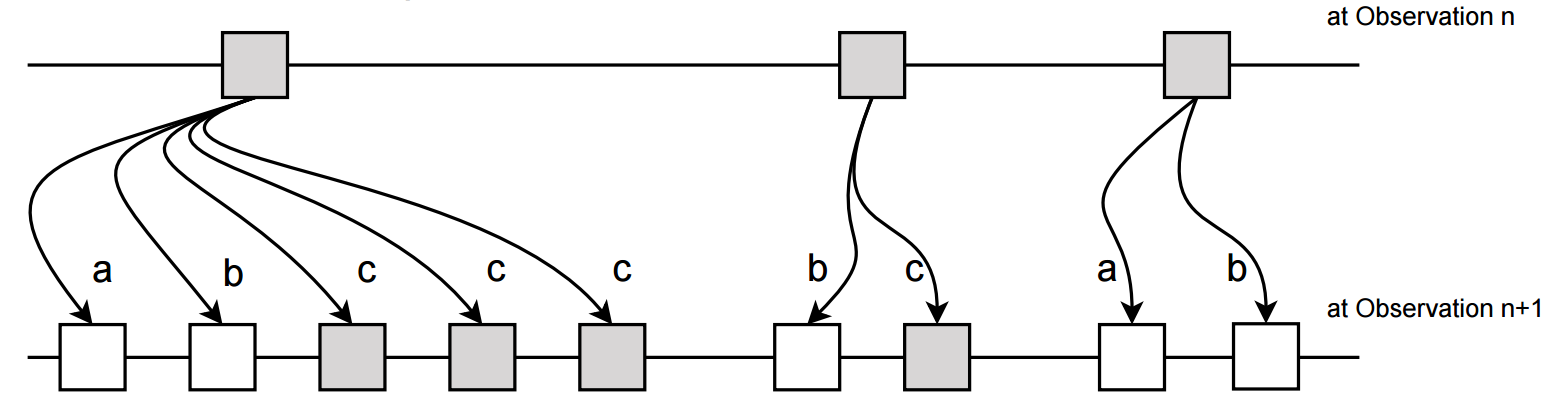
\includegraphics[scale=0.18]{diagnosis-analysis-scheme.png}
        \end{center}
        
        El estado estimado por la diagnosis será el estado que lleva la probabilidad más alta.
      \end{frame}
      
    \subsection{Predicción}
      \begin{frame}{TODO!!!}
      \end{frame}
      
    \subsection{Planificación de acciones}
      \begin{frame}{TODO!!!}
      \end{frame}

\end{document}
